\documentclass{article}
\usepackage[utf8]{inputenc}
\usepackage[a4paper, total={6.6in, 8.6in}]{geometry}
\usepackage{lastpage}
\usepackage{fancyhdr}
\usepackage[toc,page]{appendix}
\pagestyle{fancy}
\fancyhf{}
\rhead{\thepage\ of \pageref{LastPage}}
\lhead{Carroll College's AMP}
\setlength{\headheight}{12pt}
\usepackage{graphicx}
\usepackage{indentfirst}
\usepackage{float}
\usepackage{amsmath}
\usepackage{etoolbox}
\patchcmd{\thebibliography}{\section*{\refname}}{}{}{}
\usepackage{hyperref}
\hypersetup{
    colorlinks,
    citecolor=black,
    filecolor=black,
    linkcolor=black,
    urlcolor=black
}

\newcommand\decorativeline[1][1pt]{
	\par\noindent%
	\rule[0.5ex]{\linewidth}{#1}\par
}
% This is to sustain a current date without the need to change it. Please keep the file latexmkrc as is, but the timezone is changeable.
\usepackage{datetime}
\newdateformat{formatcurrentdate}{%
  \monthname[\THEMONTH] \THEDAY, \THEYEAR}
\usepackage{fontawesome5}

% Formats the table.
\usepackage[table]{xcolor}
\setlength{\arrayrulewidth}{0.0mm}
\setlength{\tabcolsep}{12pt}
\renewcommand{\arraystretch}{2.5}
% Allows a number of rows combined, adjust its column width, and insert content in its cell
\usepackage{multirow}

% Formatting the use of images
% The package to manage images
\usepackage{graphicx}
\graphicspath{ {./images/} }
\usepackage[rightcaption]{sidecap}
\usepackage{wrapfig}

% allows temporary adjustments for side margins
\usepackage{chngpage}

\begin{document}
\addtolength{\textheight}{1.25in}
\thispagestyle{empty}
\pagenumbering{gobble}
\begin{center}
\begin{minipage}{0.75\linewidth}
    \centering
    \vspace{7cm}

    {\uppercase{\Huge AMP - Athletics Music Player \par}}
    \vspace{2cm}
    by \\[\baselineskip]
    {\Large Rakiah Grende, Robert Hereth, and Elaine Schultz\par} 

    \vspace*{1\baselineskip}
    \formatcurrentdate\today

\end{minipage}
\end{center}

\clearpage
\pagenumbering{arabic}
\tableofcontents
\pagebreak

\section{UI Layout}
\quad The UI layout is for reference only and the actual UI layout shall depend on the current UI you obtain.

\subsection{UI Layout Reference}

\begin{figure}[h]
\centering
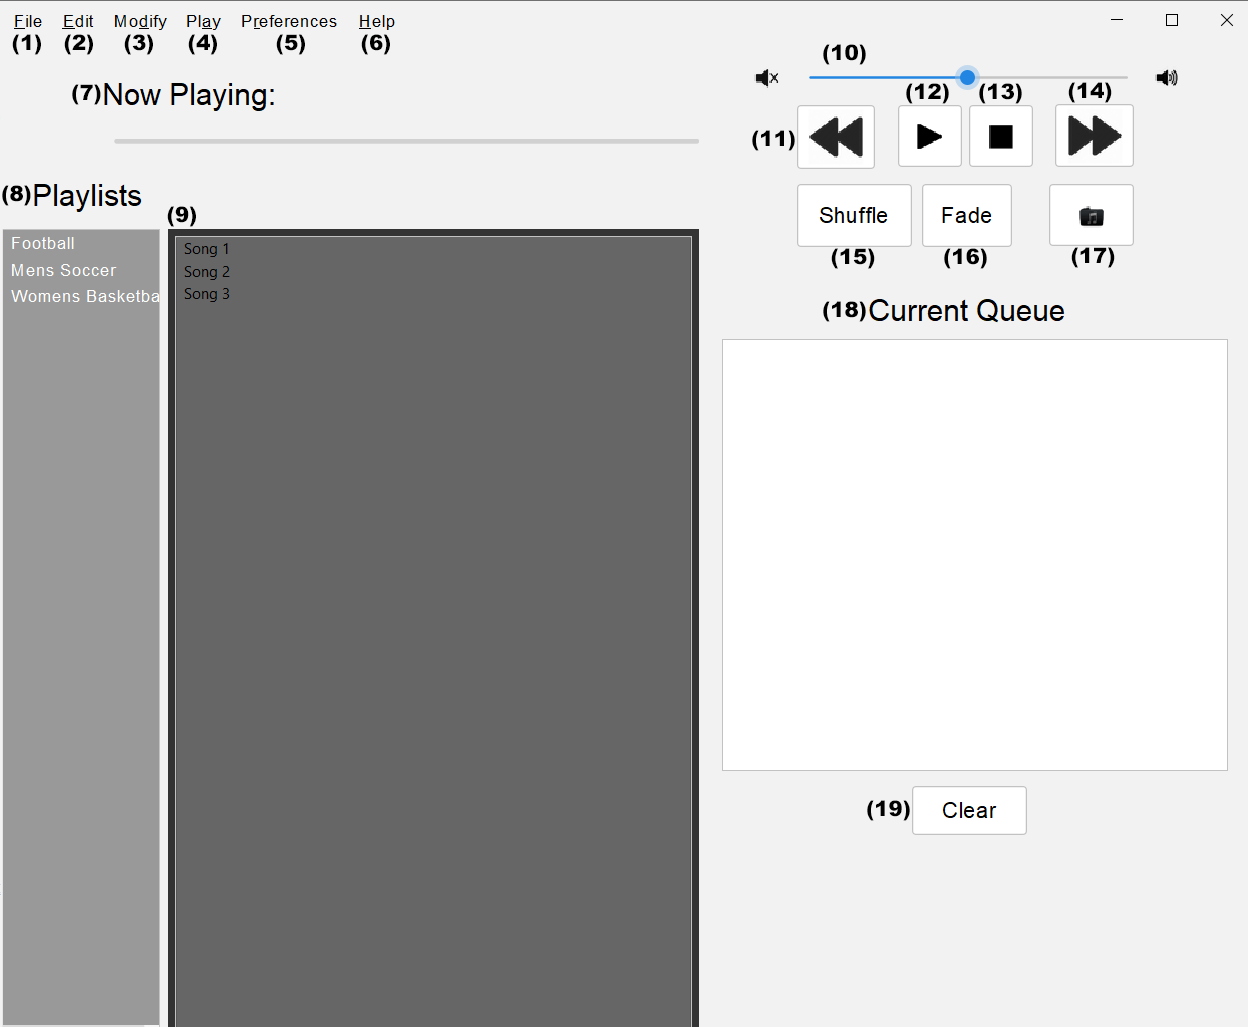
\includegraphics[width=13cm]{Images/referenceImg.png}
\end{figure}

\begin{center}
{\rowcolors{2}{black!30!gray!20}{black!20!gray!10}
\begin{tabular}{ |p{0.3cm}|p{3.3cm}|p{0.3cm}|p{3.3cm}|p{0.3cm}|p{3.3cm}| }
\hline
\multicolumn{6}{|c|}{\textbf{Reference Layout}} \\
\hline
No. & Definition & No. & Definition & No. & Definition \\
\hline
1) & File & 8) & Playlists & 15) & Shuffle \\
2) & Edit & 9) & List of Songs & 16) & Fade \\
3) & Modify & 10) & Volume & 17) & Upload Music \\
4) & Play & 11) & Backwards & 18) & Current Queue Songs \\
5) & Preferences & 12) & Play & 19) & Clears Current Queue \\
6) & Help & 13) & Stop & & \\
7) & Current Song Playing & 14) & Forward & & \\

\hline
\end{tabular}
\end{center}

\clearpage

\section{Tasks}
\quad A selection of alternative tasks for the user to perform within AMP.


\subsection{File}

\begin{itemize}
    \item[] \textbf{Create} \faIcon{angle-right}
    \begin{description}
        \item 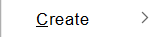
\includegraphics[width=3.5cm]{Images/File Create JMenu.png}
            \item[] Creates the following methods:
    \end{description}
    \item \textbf{Playlist}: Add new playlist.
    \begin{description}
        \item[] Create a new playlist in the playlists section:
    \end{description}
    \begin{description}
        \item 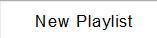
\includegraphics[width=3.5cm]{Images/File Create New Playlist.png}
    \end{description}
    \item \textbf{Tag}: Add new tag.
    \begin{description}
        \item[] Creates a new tag to note the song name, artist, and id into a playlist:
    \end{description}
    \begin{description}
        \item 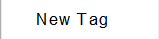
\includegraphics[width=3.5cm]{Images/File Create New Tag.png}
    \end{description}
    \item \textbf{Screen}: Add a new screen button.
    \begin{description}
        \item[] Creates and adds a new screen button:
    \end{description}
        \begin{description}
        \item 
\includegraphics[width=3.5cm]{Images/File Create New Screen.png}
    \end{description}
        \item \textbf{Song}: Add a new song.
    \begin{description}
        \item[] Creates and adds a new song to the Playlist:
    \end{description}
        \begin{description}
        \item 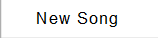
\includegraphics[width=3.5cm]{Images/File Create New Song.png}
    \end{description}
    \item \textbf{Import}: Import a music file.
    \begin{description}
        \item[] Imports an audio file:
        \item[] 
\includegraphics[width=3.5cm]{Images/File Import.png}
        \item[]Supported audio files: \faIcon{file-audio}
        \item[-]\textbf{.acc}
        \item[-]\textbf{.wav}
        \item[-]\textbf{.mp3}
    \end{description}
        \item \textbf{Exit}: Exits the Application.
    \begin{description}
        \item[] This Exits the current running application:
    \end{description}
        \begin{description}
        \item 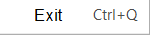
\includegraphics[width=3.5cm]{Images/File Exit.png}
    \end{description}
\end{itemize}

\subsection{Edit}

\begin{itemize}
    \item \textbf{Clip}: Edit an audio clip.
    \begin{description}
        \item[] Edit a selected audio file to adjust its time length and audio quality:
        \item 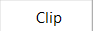
\includegraphics[width=2.5cm]{Images/Edit Clip.png}
        \item[]Supported audio files: \faIcon{file-audio}
        \item[-]\textbf{.mp3}
        \item[-]\textbf{.wav}
    \end{description}
    \item \textbf{Tag}: Edit a tag.
    \begin{description}
        \item[] Edit a created tag to change info about the song name, artist, and year:
        \item 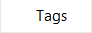
\includegraphics[width=2.5cm]{Images/Edit Tags.png}
    \end{description}
    \item \textbf{Add playlist}: Add a new playlist.
    \begin{description}
        \item[] Creates and adds a new playlist:
        \item[] 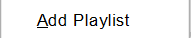
\includegraphics[width=4cm]{Images/Edit AddPlaylist.png}
    \end{description}
    \item \textbf{Remove playlist}: Remove a playlist.
        \begin{description}
        \item[] Removes a created playlist:
        \item[] 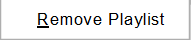
\includegraphics[width=4cm]{Images/Edit RemovePlaylist.png}
    \end{description}
\end{itemize}

\subsection{Play}
    \begin{itemize}
    \item \textbf{Select All}: Select all in Queue.
        \begin{description}
        \item[] Selects all songs from the Current Queue.
        \item[] 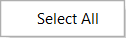
\includegraphics[width=3cm]{Images/Play Select All.png}
        \end{description}
    \end{itemize}


\subsection{Modify}

\begin{itemize}
    \item \textbf{Add song}: Add a song to a playlist.
    \begin{description}
        \item[] Adds a song into a created playlist.
        \item[] 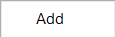
\includegraphics[width=3cm]{Images/Modify Add.png}
    \end{description}
    \item \textbf{Remove song}: Remove a song from a playlist.
    \begin{description}
        \item[] Removes a song from a created playlist.
        \item[] 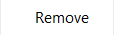
\includegraphics[width=3cm]{Images/Modify Remove.png}
    \end{description}
    \item \textbf{Search}: Search a song.
    \begin{description}
        \item[] Search a song within AMP's imported audio library:
        \item[] 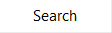
\includegraphics[width=3cm]{Images/Modify Search.png}
    \end{description}
\end{itemize}

\subsection{Preferences}

\begin{itemize}
    \item \textbf{Theme}: Changes the UI color.
    \item[] 
\includegraphics[width=3cm]{Images/Preferences_Theme.png}
    \begin{description}
        \item[] Selectable options to change the UI's color appearance.
            \item[-] Light Mode \textit{(Default UI)}
            \item[] 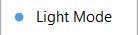
\includegraphics[width=4cm]{Images/Selected_LightMode.png}
            \item[-] Dark Mode
            \item[] 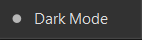
\includegraphics[width=4cm]{Images/Selected_DarkMode.png}
    \end{description}
\end{itemize}

\subsection{Help}

\begin{itemize}
    \item \textbf{Documentation}: Read and search content documentation:
    \item[] 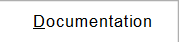
\includegraphics[width=4cm]{Images/Help Documentation.png}
    \item \textbf{About}:
    \begin{description}
        \item[] Shows what AMP is, who created the program, and information about OS and system requirements.
        \item[] 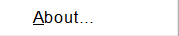
\includegraphics[width=4cm]{Images/Help About.png}
        
        \vspace{0.5cm}
        
        \item[-] \textbf{OS Support}:        
            \item[] \faIcon{apple} MacOS 10.12 Sierra, macOS 13.2.1 Ventura and above.
            \item[] \faIcon{windows} Windows 10, Windows 11 and above.
            \vspace{0.2cm}
        \item[-] \textbf{System Requirements}:

            {\rowcolors{2}{black!20!gray!10}{black!10!gray!5}
            \begin{tabular}{ |p{3cm}|p{10cm}| }
            \hline
            \multicolumn{2}{|c|}{\textbf{Minimum Specs}} \\
            \hline
            Processor & 1GHz (32-bit/64-bit), ARM Apple Silicon or ARM Processor \\
            RAM & 2GB \\
            Storage & 16GB Hard Drive Disk \\
            Graphics Card & integrated graphics \\
            Resolution & 1280x720 \\
            Sound & onboard sound \\
            \hline
            \end{tabular}

            {\rowcolors{2}{black!20!gray!10}{black!10!gray!5}
            \begin{tabular}{ |p{3cm}|p{10cm} }
            \hline
            \multicolumn{2}{|c|}{\textbf{Recommended Specs}} \\
            \hline
            Processor & 2GHz (64-bit) or above, Intel multi-core or AMD multi-core \\
            RAM & 4GB or more \\
            Storage & 32GB Solid State Drive \\
            Graphics Card & integrated graphics or dedicated graphics of 2GB or more \\
            Resolution & 1920x1080 or above \\
            Sound & onboard sound or sound card \\
            \hline
            \end{tabular}

    \end{description}
\end{itemize}

\vspace{1cm}

\section{User Interface}
\quad How to operate AMP's UI.

\subsection{Playlists}

\begin{itemize}
    \item \textbf{Top Playlist}: The top playlist.
    \begin{description}
        \item[] Displays the top playlist. This is the top-tier playlist that always remains first in the order of created playlists. Recommended to use for common-use songs.
        \item[] 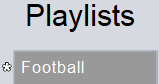
\includegraphics[width=3cm]{Images/topPlaylist.png}
    \end{description}
    \item \textbf{Playlist Name}: A selectable playlist.
    \begin{description}
        \item[] Displays a selectable playlist.
        \item[] 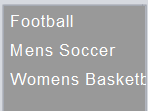
\includegraphics[width=3cm]{Images/Playlist.png}
    \end{description}
\end{itemize}

\subsection{Player Controls}

\begin{itemize}
    \item \textbf{Fade Out/In}: Fades out or fades in song.
    \begin{description}
        \item[] This fades out or fades in a song by 2 seconds for a smooth transition from the current queue song list to another song.
        \item[] 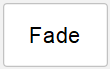
\includegraphics[width=1.5cm]{Images/Fade.png}
    \end{description}
    
    \clearpage
    
    \item \textbf{Select All}: Selects all songs.
    \begin{description}
        \item[] Pressing the button \textit{selects all} the playlist songs and moves them into the current queue:
        \item[] 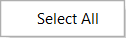
\includegraphics[width=3cm]{Images/Play Select All.png}
    \end{description}
    \item \textbf{Now Playing}: Displays playing song.
    \begin{description}
        \item[] This displays the current song running in text.
        \item[] 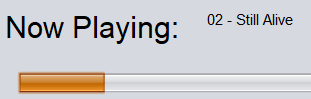
\includegraphics[width=5cm]{Images/NowPlaying.png}
    \end{description}
    \item \textbf{Play}: Plays song.
    \begin{description}
        \item[] Pressing the button \textit{plays} the current queue song:
        \item[] 
\includegraphics[width=1.5cm]{Images/Play.png}
    \end{description}
    \item \textbf{Pause}: Pauses song.
    \begin{description}
        \item[] Pressing the button \textit{pauses} the current queue song:
        \item[] 
\includegraphics[width=1.5cm]{Images/Pause.png}
    \end{description}
    \item \textbf{Stop}: Stops song.
    \begin{description}
        \item[] Pressing the button \textit{stops} the current queue song:
        \item[] 
\includegraphics[width=1.5cm]{Images/Stop.png}
    \end{description}

\end{itemize}

\subsection{List of Songs}

\begin{itemize}
    \item \textbf{[Selectable list of songs]}
        \item[] Readies a selectable list of songs collected by a preset playlist.
        \item[] 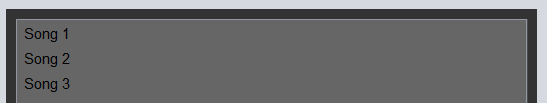
\includegraphics[width=8cm]{Images/ListOfSongs.png}
\end{itemize}

\subsection{Volume}

\begin{itemize}
    \item \textbf{Volume}: Adjusts volume.
        \item[] Adjusts the volume for the current song being played by increasing or decreasing the volume output:
        \item[] 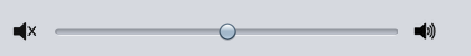
\includegraphics[width=8cm]{Images/Volume.png}
\end{itemize}

\subsection{Queue}

\begin{itemize}
    \item \textbf{[Shuffle]}: A shuffle button.
    \begin{description}
        \item[] A shuffle button that randomizes the queue's contained set of songs.
        \item[] 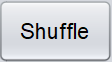
\includegraphics[width=2cm]{Images/Shuffle.png}
    \end{description}
    \item \textbf{[Queue]}: Displays the current list of songs.
        \begin{description}
        \item[] Displays the current list of songs and is ready to be operated by the player's controls.
        \item[] 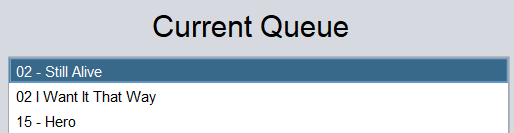
\includegraphics[width=9cm]{Images/CurrentQueue.png}
        \end{description}
\end{itemize}

\vspace{0.5cm}

\section{Database}
\quad The database mockup.

\subsection{Database Mockup}

\begin{figure}[h]
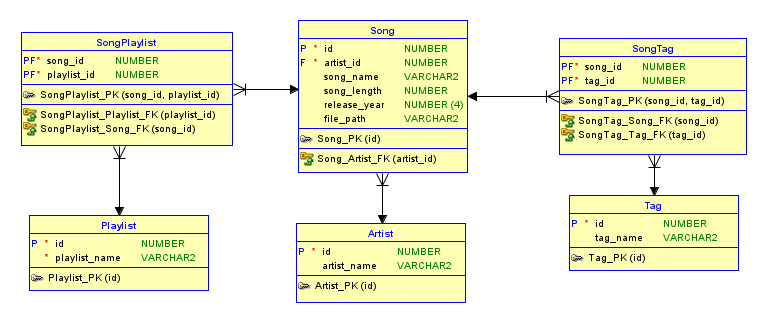
\includegraphics[width=18cm]{Images/AMP_DB_Mockup.PNG}
\end{figure}

\end{document}